%
% einleitung.tex -- Beispiel-File für die Einleitung
%
% (c) 2020 Prof Dr Andreas Müller, Hochschule Rapperswil
%
% !TEX root = ../../buch.tex
% !TEX encoding = UTF-8
%
% erste Maxwellgleichung ohne Quelle

\tikzset{>=latex} % for LaTeX arrow head
\usetikzlibrary {arrows.meta}
\pgfplotsset{compat=1.13}
\usetikzlibrary{decorations.markings,intersections,calc}
\usetikzlibrary{angles,quotes} % for pic (angle labels)
\colorlet{Ecol}{green!90!black}
\colorlet{EcolFL}{green!80!black}
\colorlet{Bcol}{blue!90!black}
\tikzstyle{EcolEP}=[blue!80!white]
\colorlet{veccol}{green!45!black}
\tikzstyle{charge+}=[very thin,top color=red!50,bottom color=red!90!black,shading angle=20]
\tikzstyle{charge-}=[very thin,top color=blue!50,bottom color=blue!80,shading angle=20]
\tikzstyle{charge_small} = [very thin,top color=red!50,bottom color=red!90,shading angle=20]
\tikzstyle{vector}=[->,thick,veccol]
\tikzset{EFieldLineArrow/.style={EcolFL,decoration={markings,mark=at position #1 with {\arrow{latex}}},
		postaction={decorate}},
	EFieldLineArrow/.default=0.5}


\section{Elektrostatik\label{maxwell:section:elekktrostatik}}
\rhead{Elektrostatik}
Die Elektrostatik ist ein Spezialfall der Elektrodynamik, bei dem statische Felder betrachtet werden.
Dies setzt voraus, dass
\begin{equation}
	\frac{\partial f}{\partial t}
	=
	0
	\qquad
	\forall f,t.
	\label{maxwell:section:definition_statik}
\end{equation}
Daraus folgt, dass wir nur ruhende Ladungen betrachten.
Dies hat zur Folge, dass keine Stromdichten existieren können, weil
\begin{equation}
	\rho\,\vec{v}
	=
	\rho\, \underbrace{\frac{\partial \vec{x}}{\partial t}}_{=0}
	=
	\vec{j}
	=
	0.
\end{equation}
Im späteren Abschnitt \ref{maxwell:magnetostatik} der Magnetostatik wird klar, dass aus diesem Grund in der Elektrostatik keine magnetische Flussdichte existieren kann.
 
Das Ziel ist nun das elektrische Feld im Zusammenspiel mit ruhenden Ladungen zu beschreiben.
Dafür werden wir in den folgenden Abschnitten die nötigen Begriffe definieren und genauer erklären.

\subsubsection{Elektrisches Potentialfeld}
Das elektrische Potentialfeld
\[
\phi:\mathbb{R}^3
\rightarrow
\mathbb{R}
\]
ist als
\begin{equation}
	\phi(x,y,z)
	=
	\frac{W_{pot}(x,y,z)}{q}
	\label{maxwell:section:definition_elektrischespotentialfeld}
\end{equation}
definiert.
In Worten gefasst kann man sagen, dass das elektrische Potential eine auf die Ladung normierte, potentielle Energie darstellt.
Somit kann die linke Abbildung in \ref{maxwell:skalarGrad} als ein Feld, das proportional zur potentiellen Energie ist, angeschaut werden.
Des Weiteren steht die elektrische Spannung eng in Verbindung mit dem elektrischen Potential.
Die Spannung $U$ zwischen zwei Punkten $a$ und $b$ wird definiert als
\[
U_{ab}
=
\phi_a - \phi_b.
\]
% not sure about this
Das heisst die Spannung ist der Potentialunterschied zwischen zwei Punkten.

\subsubsection{Elektrisches Feld}
Das elektrische Feld
\[
\vec{E}:\mathbb{R}^3 \rightarrow \mathbb{R}^3
\]
wird ganz allgemein definiert als
\begin{equation}
\vec{E}(x,y,z)
=
- \nabla\phi(x,y,z) - \frac{\partial \vec{A}}{\partial t}(x,y,z),
\label{maxwell:section:definiton_allgemein_elektrischesFeld}
\end{equation}
wobei $\vec{A}$ das magnetische Vektorpotential ist \eqref{maxwell:definitionVektorpot}.
Da wir dank Gleichung \eqref{maxwell:section:definition_statik} wissen, dass alle zeitlichen Ableitungen null sein müssen, ist die statische Definition des elektrischen Feldes
\begin{equation}
\vec{E}
=
- \nabla\phi.
\label{maxwell:section:definition_statisch_elektrischesFeld}
\end{equation}
Diese Definition besagt, dass das elektrische Feld ein statisches Gradientenfeld ist.
Dieses Feld kann man anhand der Kraftwirkung an sogenannten Probeladungen $q$ messen, da
\[
\vec{E}
=
\frac{\vec{F}}{q}
\]
ist.
Somit sind die Vektoren in Abbildung \ref{maxwell:section:E-Feld_punktladung} Kraft Vektoren, welche normiert sind auf die Ladung $q$.
%E-Field of point charge
\begin{figure}
	\centering
	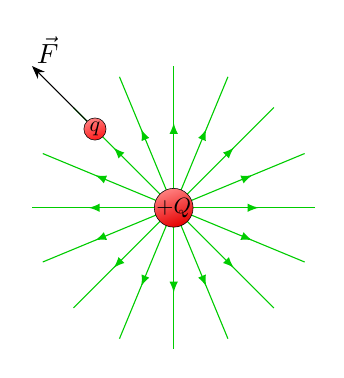
\begin{tikzpicture}
		\def\R{1.8}
		\def\NE{16}
		\def\NV{4}
		\contourlength{1.6pt}
		
		\foreach \i [evaluate={\angle=(\i-1)*360/\NE;}] in {1,...,\NE}{
			\draw[EFieldLineArrow={0.6}] (0,0) -- (\angle:\R);
		}
		\draw[charge+] (0,0) circle (7pt) node[black,scale=0.8] {$+Q$};
		%\draw[FFieldLineArrow={0.6}] (-1,1) -- (-2,2);
		\draw[-{Stealth[black]}] (-1,1) -- (-1.8,1.8) node at (-1.6, 2) {$\vec{F}$};
		\draw[charge_small] (-1,1) circle (4pt) node[black,scale=0.8] {$q$};
	\end{tikzpicture}
	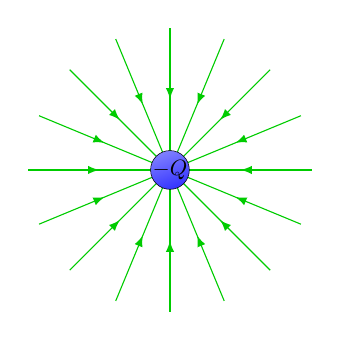
\begin{tikzpicture}
		\def\R{1.8}
		\def\NE{16}
		\def\NV{4}
		\contourlength{1.6pt}
		
		\foreach \i [evaluate={\angle=(\i-1)*360/\NE;}] in {1,...,\NE}{
			\draw[EFieldLineArrow={0.5}] (\angle:\R) -- (0:0);
		}
		\draw[charge-] (0,0) circle (7pt) node[black,scale=0.8] {$-Q$};
	\end{tikzpicture}
	\caption{Elektrisches Feld einer positiven Punktladung}
	\label{maxwell:section:E-Feld_punktladung}
\end{figure}

\subsubsection{Energiedichte im elektrischen Feld}
Das elektrische Feld beinhaltet eine Energie und somit auch eine Energiedichte.
Diese Energiedichte ist definiert als
\begin{equation}
w_e
=
\frac{1}{2}\,\epsilon\,\vec{E}\,^2,
\label{maxwell:section:definiton_energiedichte_elektrischesFeld}
\end{equation}
wobei $\epsilon$ die Permittivität ist.
Die Permittivität
\[
\epsilon
=
\epsilon_r\,\epsilon_0
\]
ist ein Mass dafür wie gut sich ein Material polarisieren lässt und ist das Produkt der relativen Permittivität $\epsilon_r$ und der Permittivität von Vakuum $\epsilon_0$.
Die relative Permittivität ist eine materialabhängige Grösse und hat in Vakuum den skalaren wert $1$.
Die Permittivität von Vakuum
\[
\epsilon_0
=
8.854 \cdot 10^{-12} F/m
\]
ist die elektrische Feldkonstante.


\subsection{Gausssches Gesetz quellenfrei
	\label{maxwell:section:elektrostatik_ohne_quelle}}
\rhead{Problemstellung}
Man stelle sich nun einen ladungsfreien, luftleeren, drei dimensionalen Raum $V\subset\mathbb{R}^3$
vor, indem ein elektrisches Potentialfeld $\phi(x,y,z)$ existiert.
Für diesen Raum möchten wir mittels der Varitaionsrechnung eine Gleichung entwickeln, die beschreibt, wie sich das Potentialfeld verhählt. 

\subsubsection{Ansatz}
Damit wir eine Gleichung erhalten, die das Verhalten des elektrischen Potentialfeldes beschreibt, muss ganz allgemein die Energie im System minimiert werden. 
In diesem Fall ist die Energie im System
\[
W_e
=
\iiint_V w_e\, dV.
\]
Dieses Integral gilt es zu minimieren, was die Grundlage für unser Variationsproblem darstellt.
Die in \eqref{maxwell:section:definiton_energiedichte_elektrischesFeld} definierte Energiedichte ist in Vakuum
% TODO: Bei definitionen erwähnen, dass ein vektor v^2 = v dot v ist!
\[
w_e\
=
\frac{1}{2}\,\epsilon_0\,\vec{E}\,^2.
\]
Diese Gleichung können wir nun mittels definition \eqref{maxwell:section:definition_statisch_elektrischesFeld} mit dem elektrischen Potentialfeld ausdrücken.
somit ist
\begin{align}
\renewcommand{\arraystretch}{1.9}
w_e
&=
\frac{1}{2}\,\epsilon_0\left(-\nabla\phi\right)^2
\\
w_e
&=
\frac{1}{2}\,\epsilon_0
\begin{pmatrix}
\displaystyle
-\phi_x\\
\displaystyle
-\phi_y\\
\displaystyle
-\phi_z
\end{pmatrix}
\cdot
\begin{pmatrix}
\displaystyle
-\phi_x\\
\displaystyle
-\phi_y\\
\displaystyle
-\phi_z
\end{pmatrix}
\\
w_e
&=
\frac{1}{2}\,\epsilon_0\left(\phi_x^2 + \phi_y^2 + \phi_z^2\right).
\label{maxwell:section:energiedichte}
\end{align}
Dies können wir in das zu minimerende Integral einsetzen und bekommen
%TODO: eventuell underbraces weg lassen.
\begin{equation}
	W_e
	=
	\iiint_V \underbrace{
		\frac{1}{2}\,\epsilon_0\left(\phi_x^2 + \phi_y^2 + \phi_z^2\right)}_{L(x,y,z,\phi,\phi_x,\phi_y,\phi_z)}\, dV.
	\label{maxwell:section:energieintegral_quellenfrei}
\end{equation}
Aus dieser Gleichung können wir entnehmen, dass unsere Lagrangefunktion
\begin{equation}
	L(x,y,z,\phi,\phi_x,\phi_y,\phi_z)
	=
	\frac{1}{2}\,\epsilon_0\left(\phi_x^2 + \phi_y^2 + \phi_z^2\right)
	\label{maxwell:section:lagrangefunktion_quellenfrei}
\end{equation}
ist.
Somit haben wir unsere Lagrangefunktion gefunden, die wir in einem nächsten Schritt in die Euler-Ostrogradski-Differentialgleichung einsetzen können.

\subsubsection{Einsetzen in die Euler-Ostrogradski-Differentialgleichung}
%TODO: label suchen von E-O-DGL von müller kapitel
Nun gilt es die in \eqref{maxwell:section:lagrangefunktion_quellenfrei} gefundene Gleichung in die E-O-DGL \ref{???} einzusetzen.
Nach Einsetzen wird die Differentialgleichung
\[
\frac{1}{2}\,\epsilon_0\left(\underbrace{\frac{\partial}{\partial\phi}\left(\phi_x^2 + \phi_y^2 + \phi_z^2\right)}_{=0} - \frac{\partial}{\partial x}\frac{\partial}{\partial \phi_x}\left(\phi_x^2 + \phi_y^2 + \phi_z^2\right) - 
\frac{\partial}{\partial y}\frac{\partial}{\partial \phi_y}\left(\phi_x^2 + \phi_y^2 + \phi_z^2\right) - 
\frac{\partial}{\partial z}\frac{\partial}{\partial \phi_z}\left(\phi_x^2 + \phi_y^2 + \phi_z^2\right)\right)
=
0.
\]
Man sieht, dass die partielle Ableitung nach $\phi$ verschwindet.
Nach den partiellen Ableitungen nach $\phi_x$, $\phi_y$ und $\phi_z$ wird die Differentialgleichung
\[
\frac{1}{2}\,\epsilon_0\left(-\frac{\partial}{\partial x}2\phi_x - \frac{\partial}{\partial y}2\phi_y - \frac{\partial}{\partial z}2\phi_z\right)
=
0.
\]
Wenn man nun noch die letzten partiellen Ableitungen macht, wird die Differentialgleichung
\begin{equation}
	- \underbrace{\epsilon_0}_{\not{=}0}\underbrace{\left(\frac{\partial^2\phi}{\partial x^2} + \frac{\partial^2\phi}{\partial y^2} + \frac{\partial^2\phi}{\partial z^2}\right)}_{=0}
	=
	0.
	\label{maxwell:section:laplace_gleichung_1}
\end{equation}
%definiton des laplace operators suchen
An dieser Gleichung sieht man, dass die Klammer mit den partiellen Ableitungen gleich null sein muss, da die Permittivität von Vakuum nicht null sein kann.
Zusätzlich wird nun ersichtlich, dass der Klammerterm nach definition \ref{???} mit dem Laplace-Operator angewendet auf das elektrische Potentialfeld $\phi$ ersetzt werden kann.
Somit wird unsere schluss Differentialgleichung
\begin{equation}
	\Delta\phi
	=
	0.
	\label{maxwell:section:laplace_gleichung_2}
\end{equation}
Durch Anwendng der Definiton des Laplace-Operator \ref{???} und der Definiton des elektrischen Feldes \eqref{maxwell:section:definition_statisch_elektrischesFeld} erhalten wird die Gleichung
\[
\nabla\cdot\underbrace{\nabla\phi}_{-\vec{E}}
=
0.
\]
Hiermit erhalten wir, dass
\begin{equation}
	\nabla\cdot\vec{E}
	=
	0
	\label{maxwell:section:e_feld_quellenfrei}
\end{equation}
% TODO:Bild referenz einfügen und Bild erstellen
sein muss. Diese Differentialgleichung besagt, dass das elektrische Feld quellenfrei ist.
Dies bedeutet, dass Felldlinien des elektrischen Feldes an keinem Ort im Raum enstehen oder enden können.
Dies ist sehr naheliegend, da ohne Ladungen im Raum das elektrische Feld quellenfrei sein muss.

%Darf auch weggelassen werden.
\subsubsection{Exkurs zur Laplace-Gleichung}
\label{maxwell:section:laplacegleichung_exkurs}
Ein Potentialfeld, das die Laplace-Gleichung
\[
-\Delta\varphi
=
0
\]
erfüllt, führt zu einem Gradientenfeld $\nabla\varphi$, das rotationsfrei und quellenfrei ist.
Diese Gleichung findet nicht nur Anwendungen in der Elektrostatik, sondern auch in stationärer Fluiddynamik und stationärer Wärmeleitung.






